\documentclass[12pt]{article}

\usepackage{amsmath,amssymb,amsthm}
\usepackage{geometry}
\usepackage{enumerate}
\usepackage[shortlabels]{enumitem}
\usepackage{graphicx}

\usepackage{hyperref}

\begin{document}
\title{CS 6965 Advanced Data Visualization\\{\bf Project 4}}
\author{Yulong Liang (u1143816)}
\maketitle

\section*{Step 1: Getting Started (4 points)}
\begin{itemize}
\item Wechat Red Envelopes I have ever received and handed out.
\item Wechat transaction data can only be accessed via Wechat mobile app and there are no export methods. I can only copy and paste the data as plain text and then do further cleaning and processing to get structured data.
\item I can keep balance between receiving and handing out money to avoid losing too much money or too many friends. I can also recognize the ones who care about me the most and the ones who I care the most.
\item The comparison between the amount of money sent and received. The top five in sending me money and top five in receiving my money.
\end{itemize}

\section*{Step 2: Design Process (3 points)}
\begin{itemize}
\item Virtual Reality. It is a virtual data phisicalization which provide people a experience as if he or she was in that space. It is also easy to demostrate things that is not feasible in real world.
\item Aggregating the money received and handed out by day and calculating the cumulative summation. Aggregating the money received by sender and ranking by summation. Generating coordinates by the date and total money so that it can be used by \texttt{MEL} in Autodesk Maya.
\item Whether will the experience be interesting enough to leave the user a great impression.
\end{itemize}

\section*{Step 3: Creating the Physical Visualization (8 points)}
\begin{itemize}
\item The comparison between the amount of money sent and received. The top six in sending me money. I can't know who received my money because the records are not listed in the transations.
\item Drawing two metal tubes which form a spiral to denote money received and handout over years. Drawing figures standing on gold bricks to denote the friends who sent me a lot of money. Placing camera in the middle of the space to view the whole space.
\item The photos are as follows:
\begin{figure}[h]
\centering
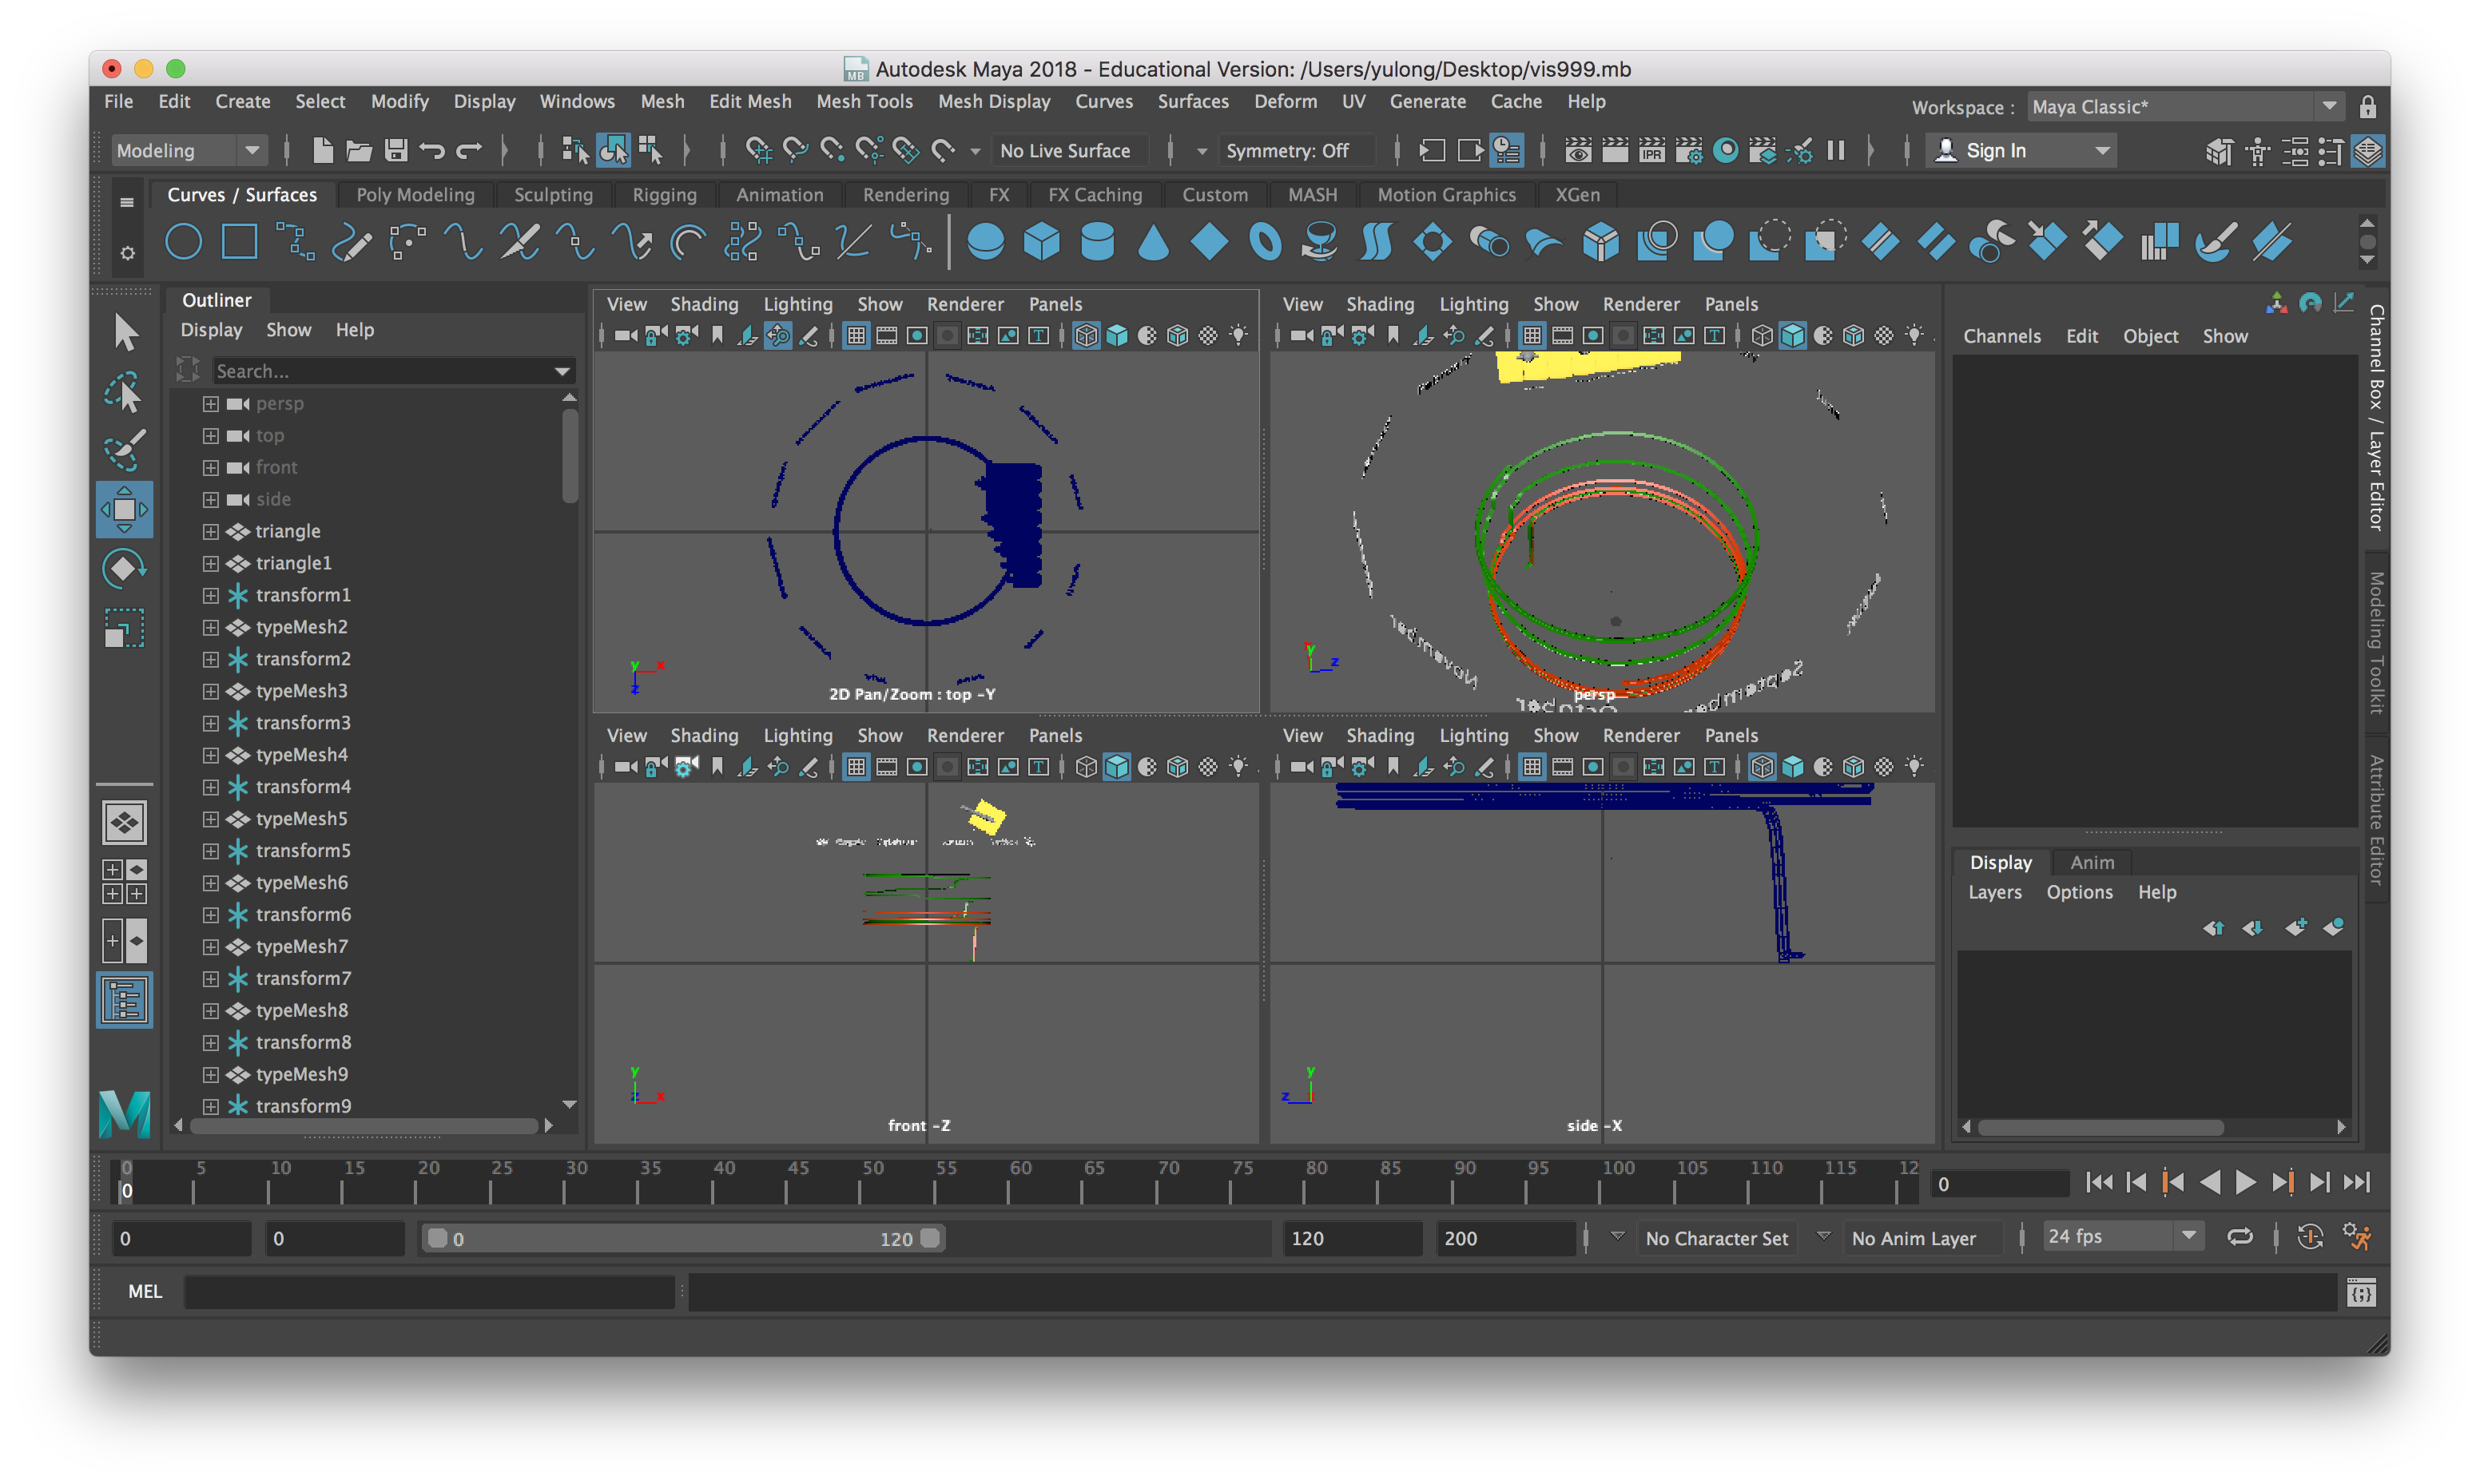
\includegraphics[width=.8\linewidth]{1.png}
\caption{Virtual Reality Space Modelling with Autodesk Maya}
\label{fig:name}
\end{figure}
\begin{figure}[h]
\centering
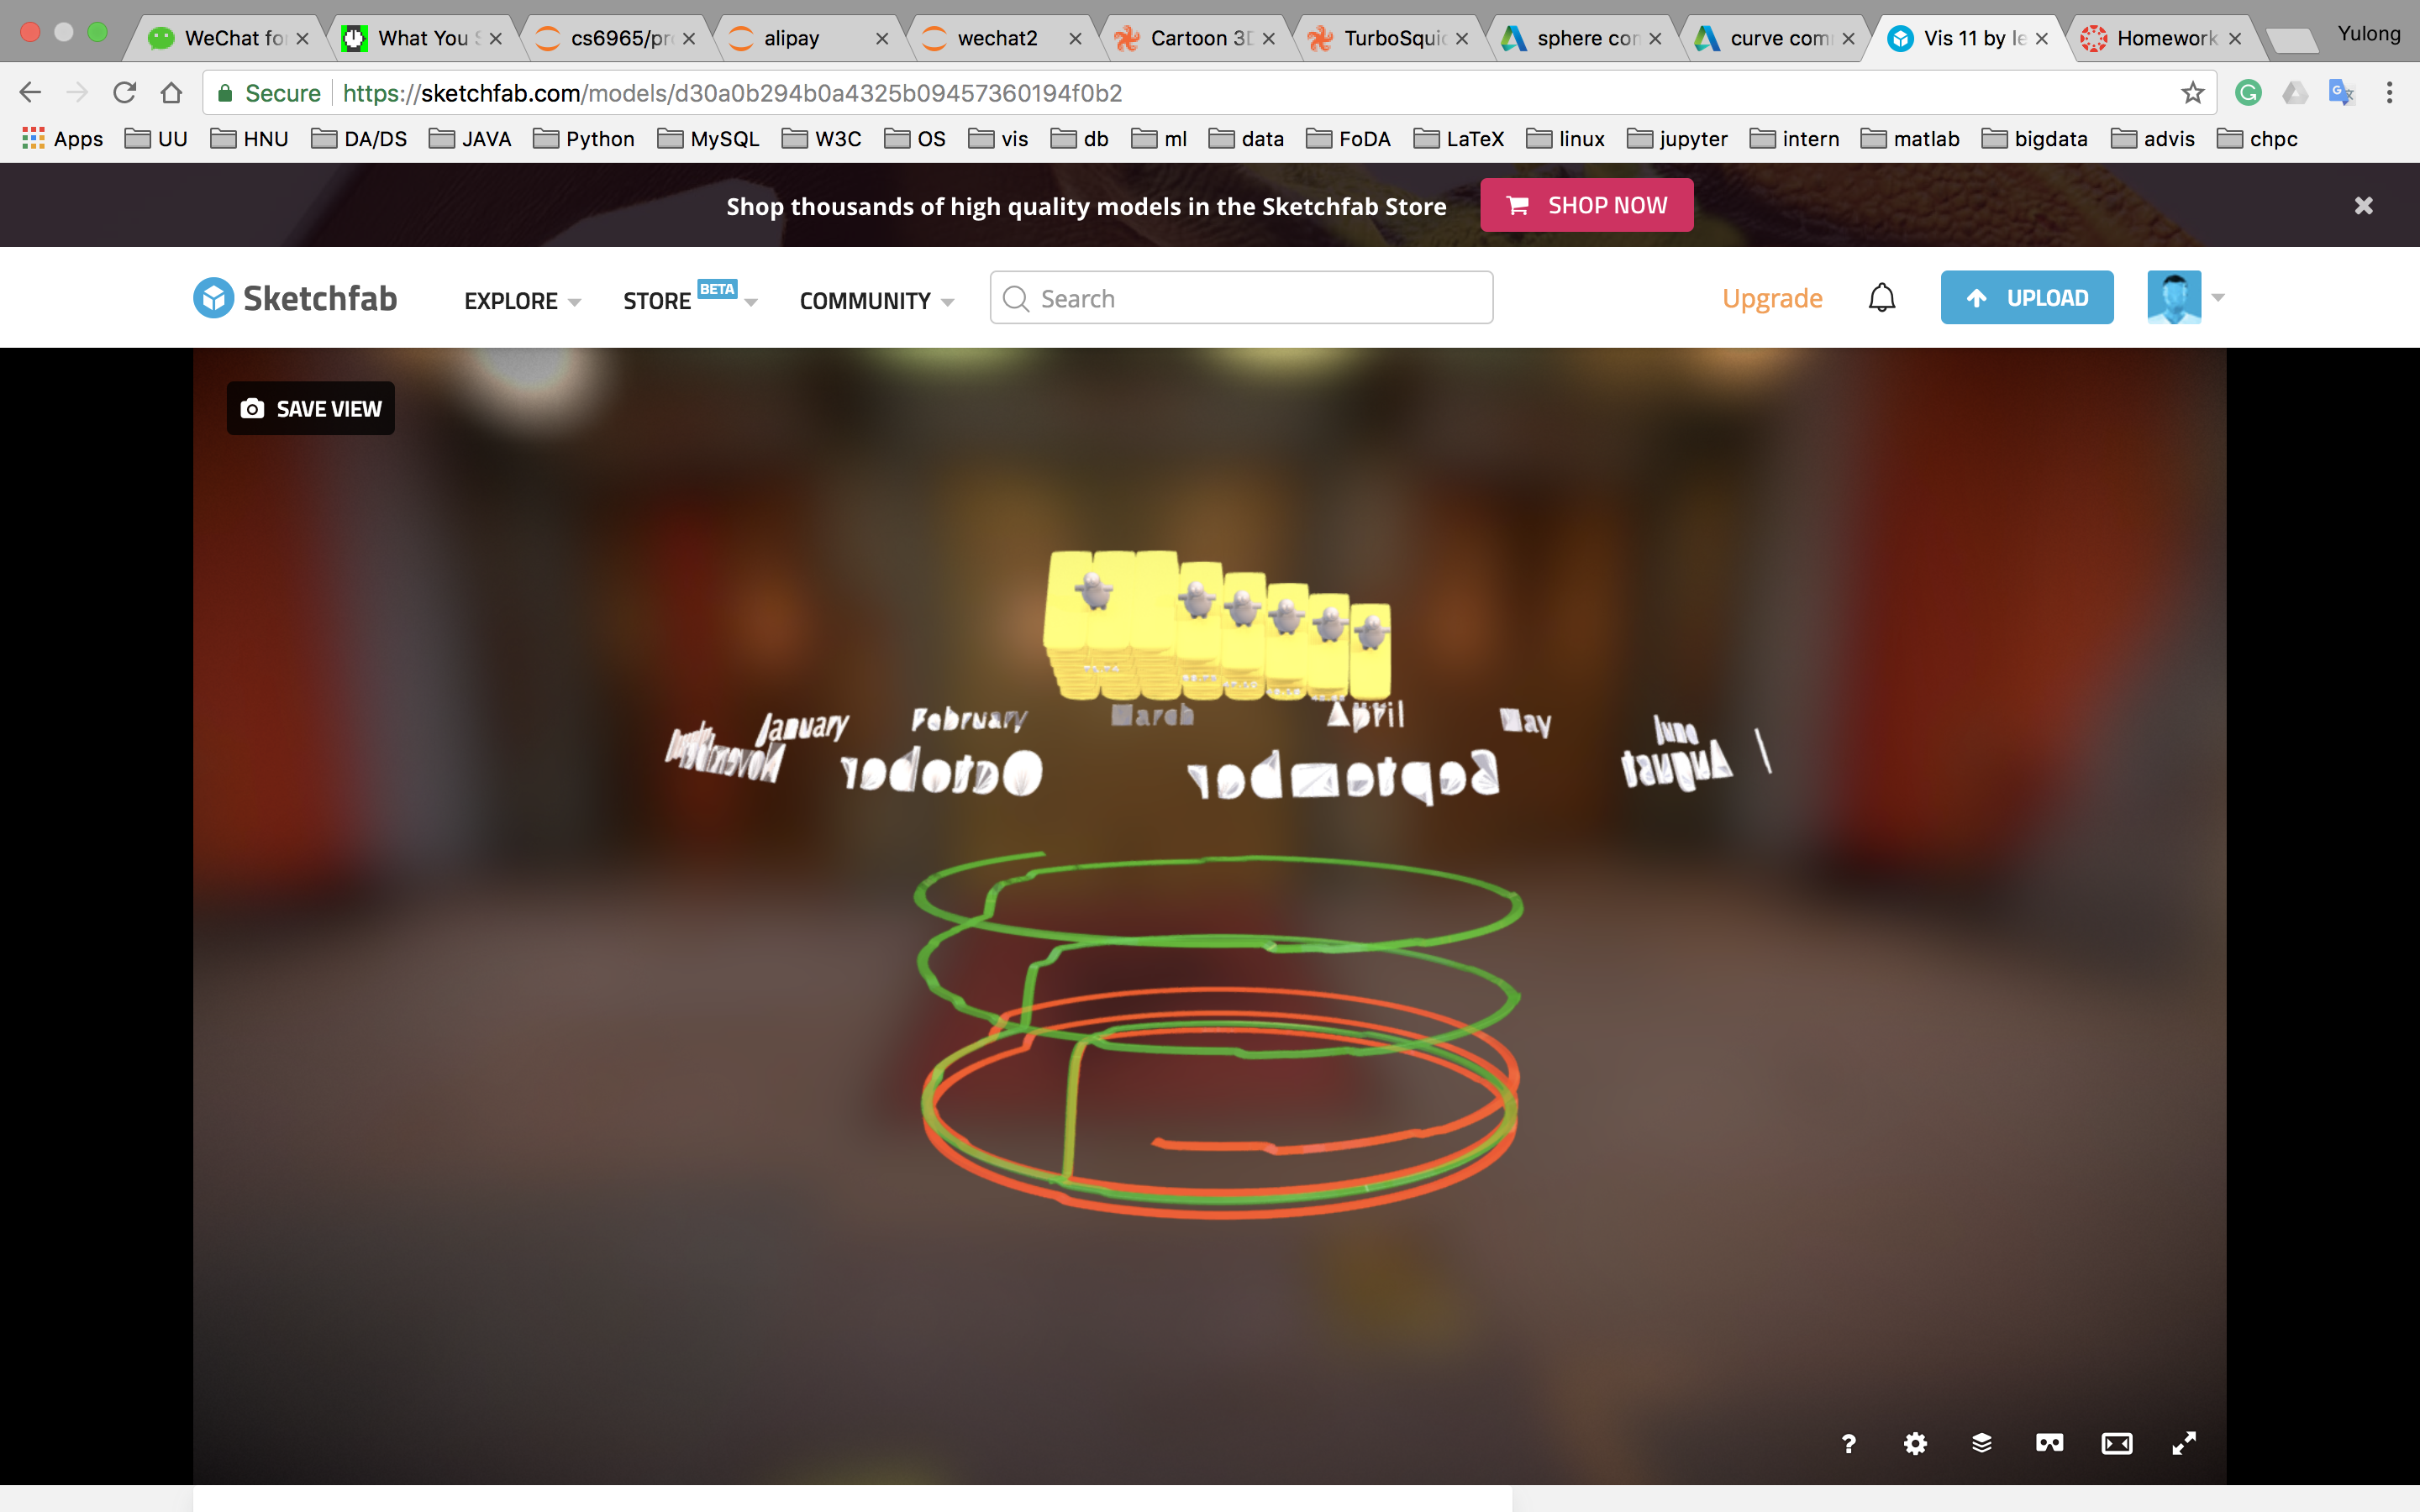
\includegraphics[width=.8\linewidth]{2.png}
\caption{Standard View of the 3D Space on Sketchfab.com}
\label{fig:name}
\end{figure}
\begin{figure}[h]
\centering
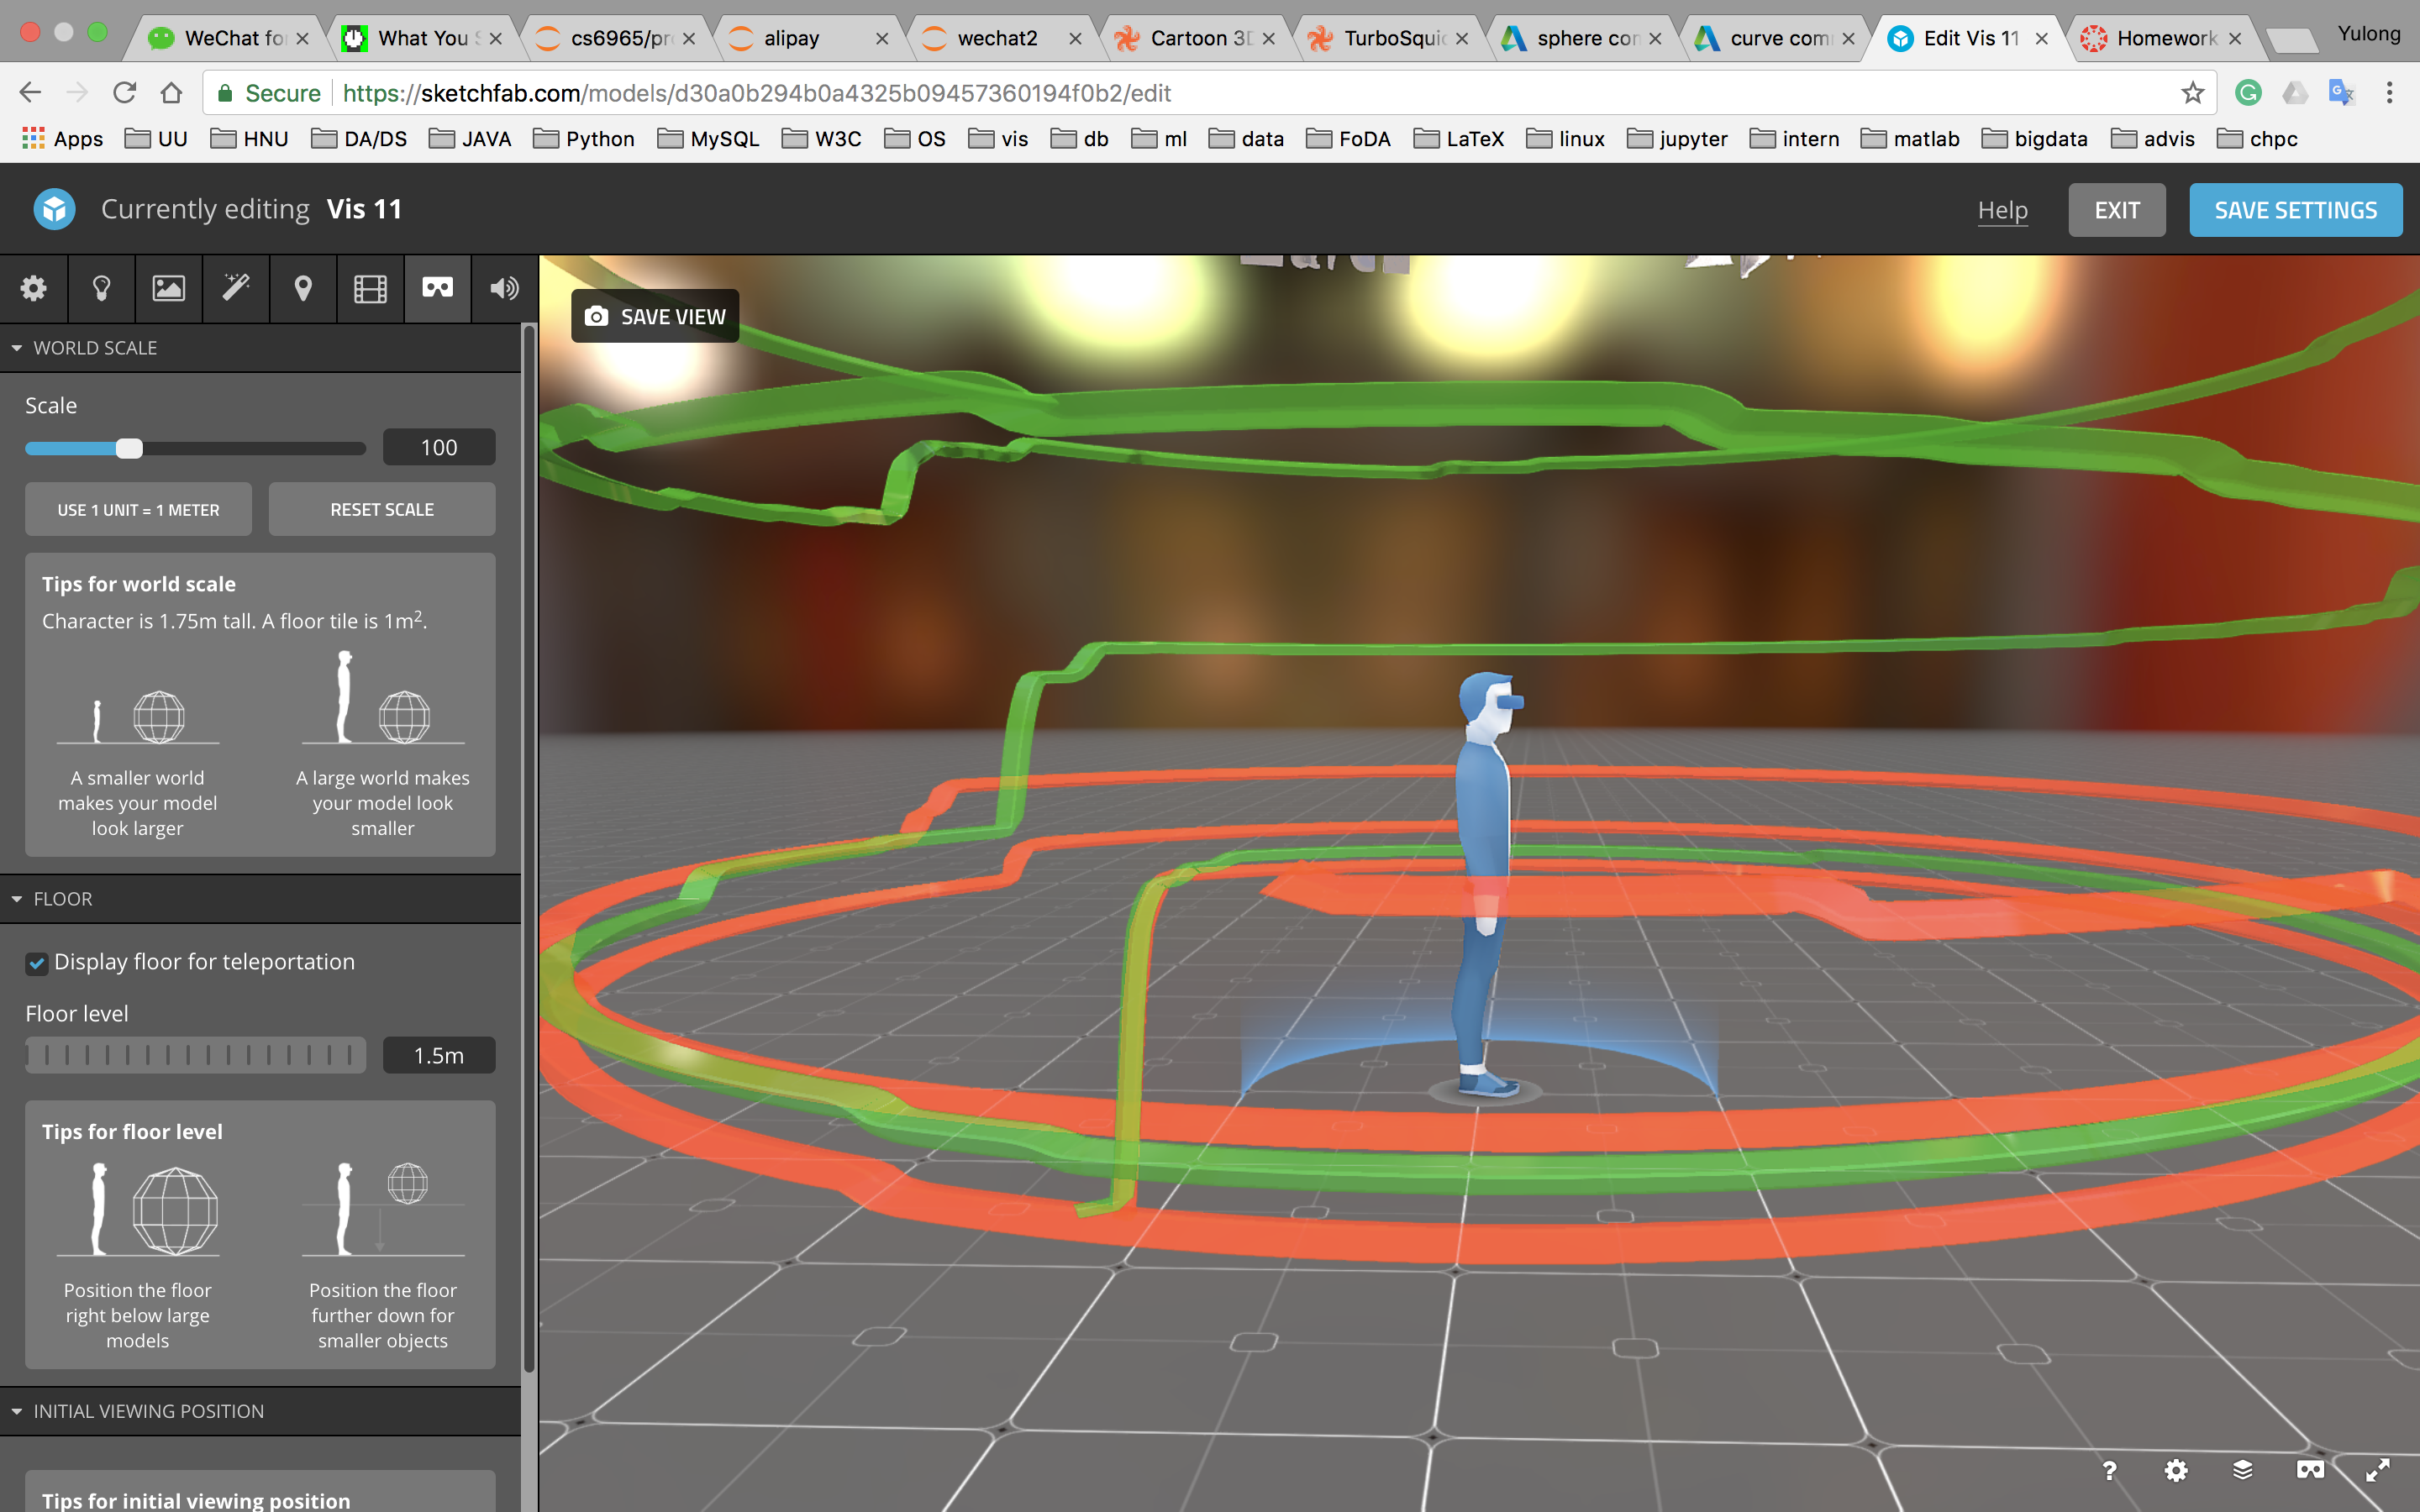
\includegraphics[width=.8\linewidth]{3.png}
\caption{Virtual Reality View of the 3D Space on Sketchfab.com}
\label{fig:name}
\end{figure}
\begin{figure}[h]
\centering
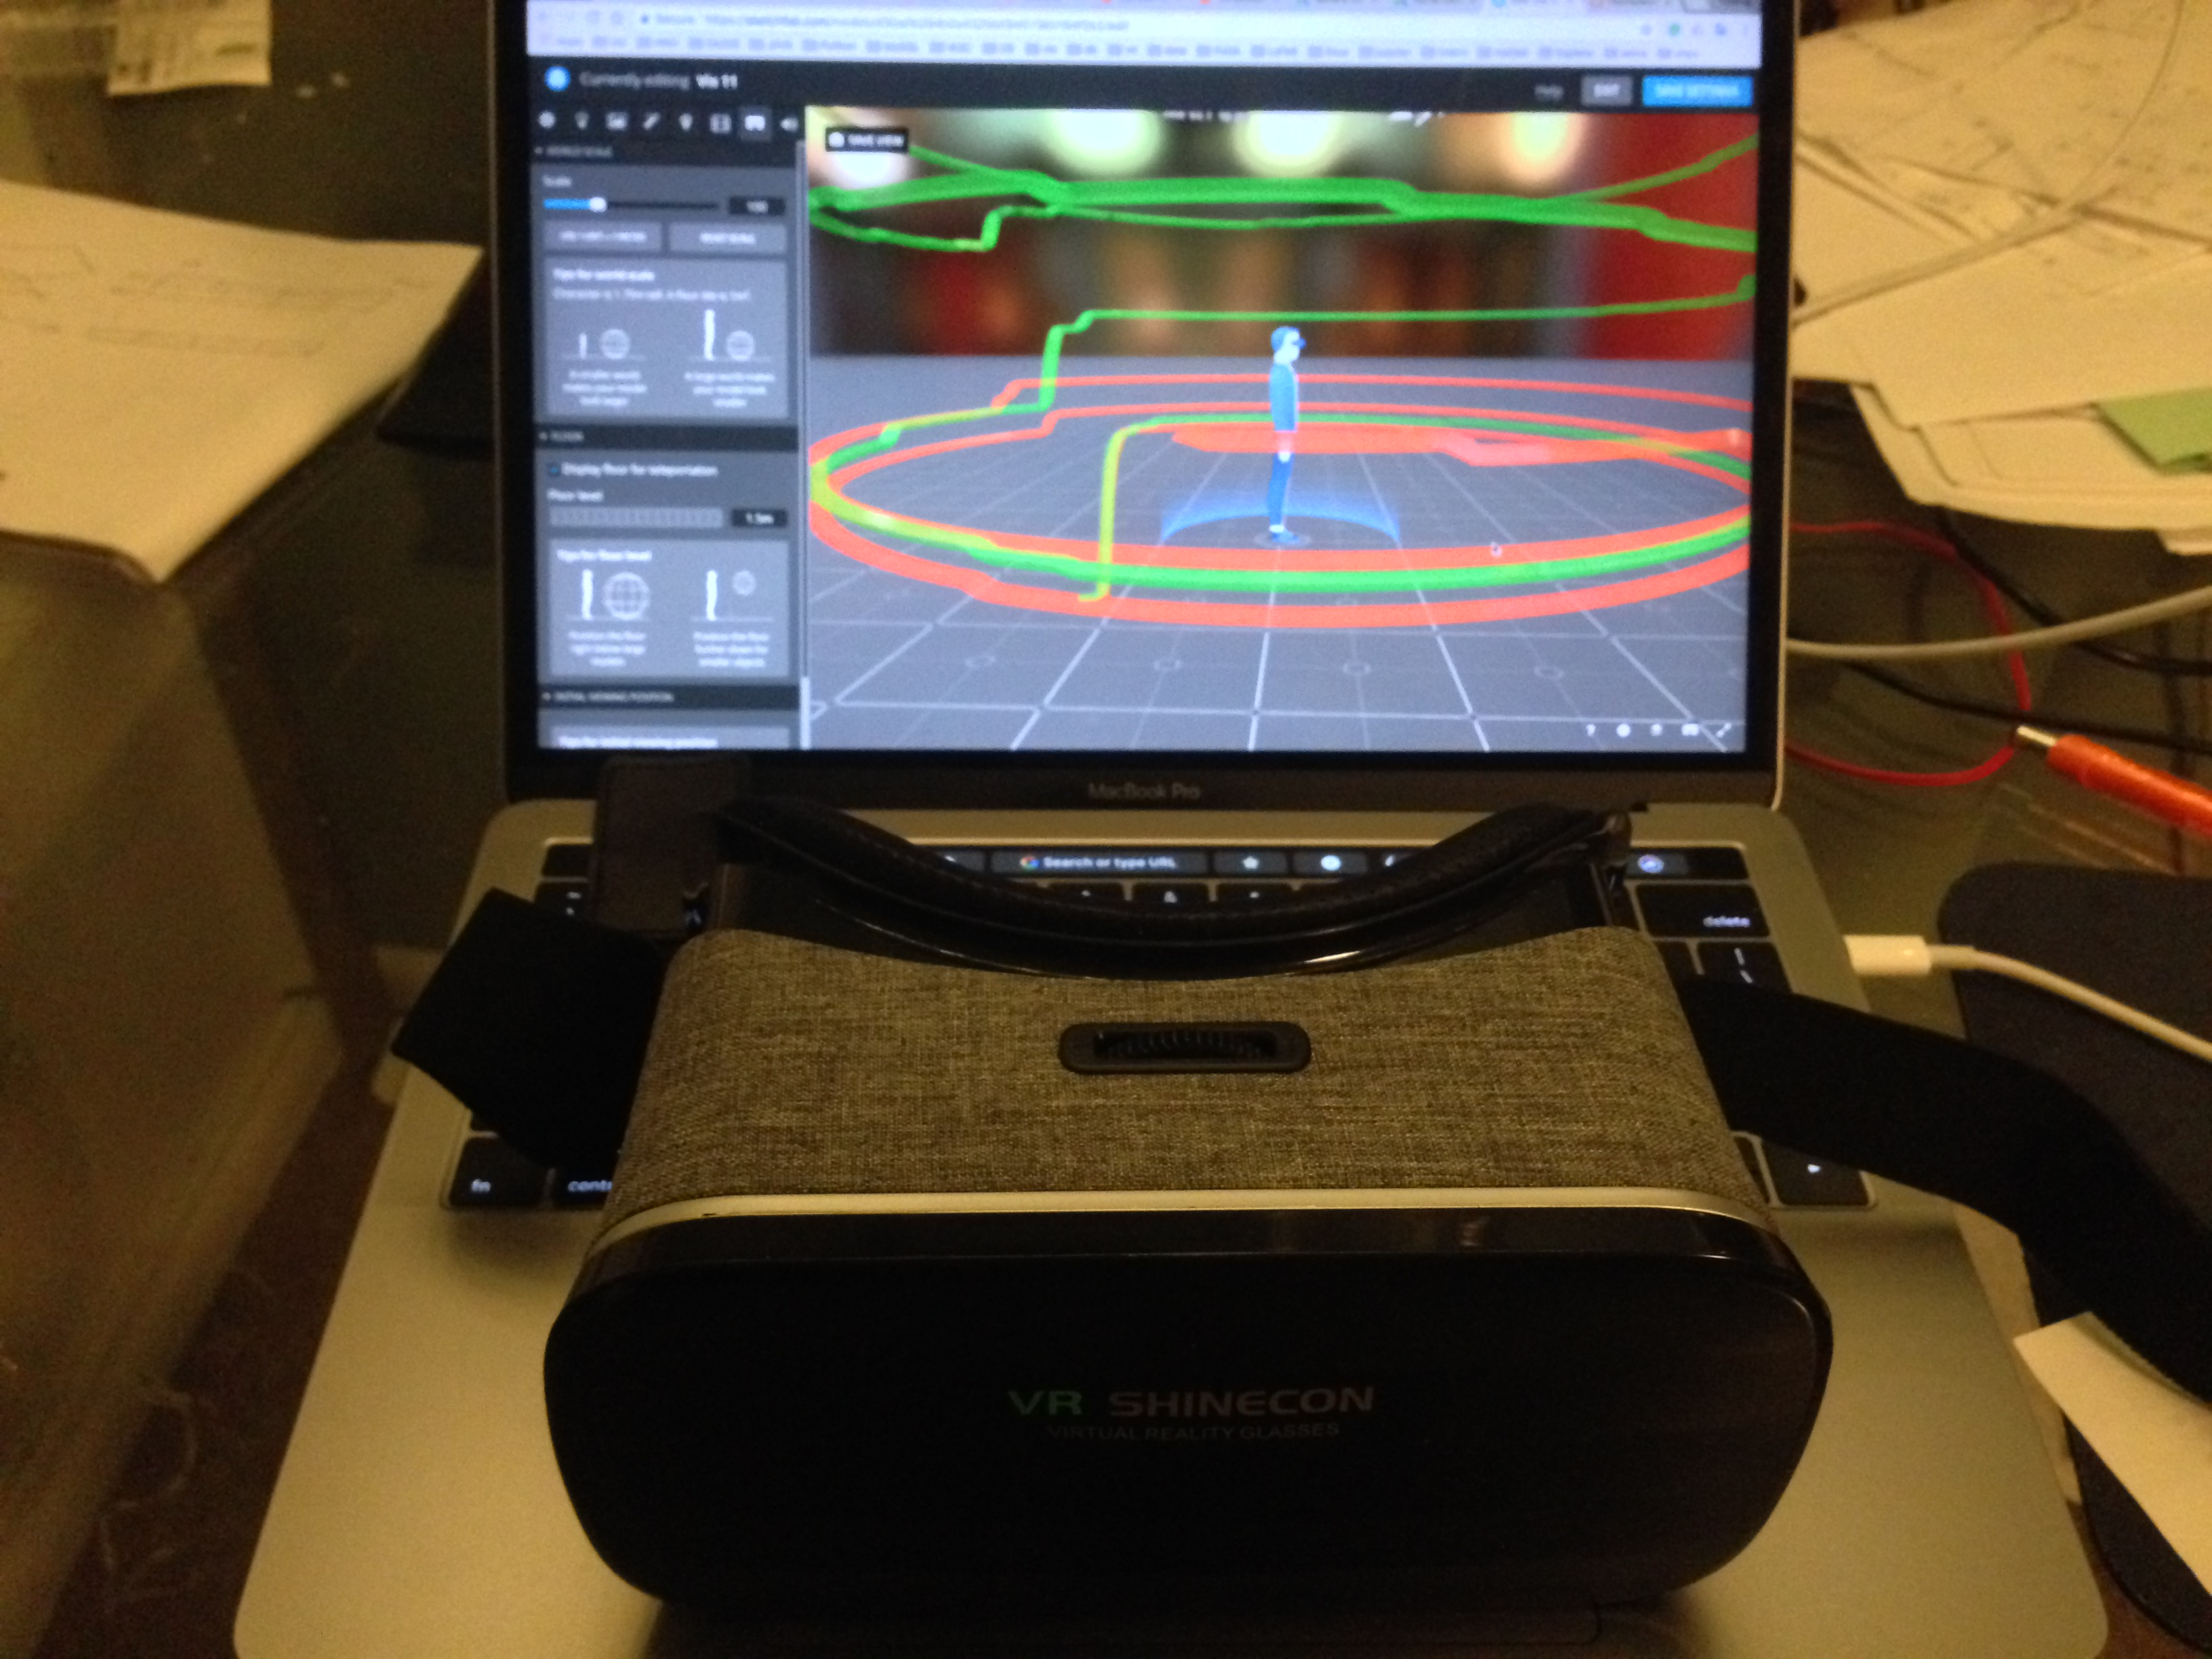
\includegraphics[width=.8\linewidth]{4.jpg}
\caption{Virtual Reality Gear - Cardboard}
\label{fig:name}
\end{figure}
\end{itemize}


\end{document}